\section{初识上手 Power BI}

\subsection{安装和运行}

\textbf{方法一:}如\figref{fig:download_powerbi}中所示,前往\url{https://powerbi.microsoft.com/zh-cn/desktop/},选择``免费下载''(会请求跳转至Microsoft Store)。或直接在Microsoft Store中搜索并下载Power BI Desktop产品。该方法的一个好处是,当Power BI Desktop更新时,可以后台自动更新且无须重新下载安装。

\begin{figure}[htbp]
    \centering
    
\includegraphics[width=0.9\textwidth]{figure/PowerBI/download_powerbi.png}
    \caption{\textbf{在Microsoft Store中下载Power BI Desktop(此处为从官网跳转进入)}}
    \label{fig:download_powerbi}
\end{figure}

\textbf{方法二:}如\figref{fig:download_powerbi_web}中所示,前往\url{https://www.microsoft.com/zh-CN/download/details.aspx?id=58494}(可从方法一的网页中选择``查看下载或语言选项''进入到本网页),选择语言后,点击``下载'',并根据电脑的硬件需求选择下载64位版本或32位版本的Power BI Desktop安装包。

\begin{figure}[htbp]
    \centering
    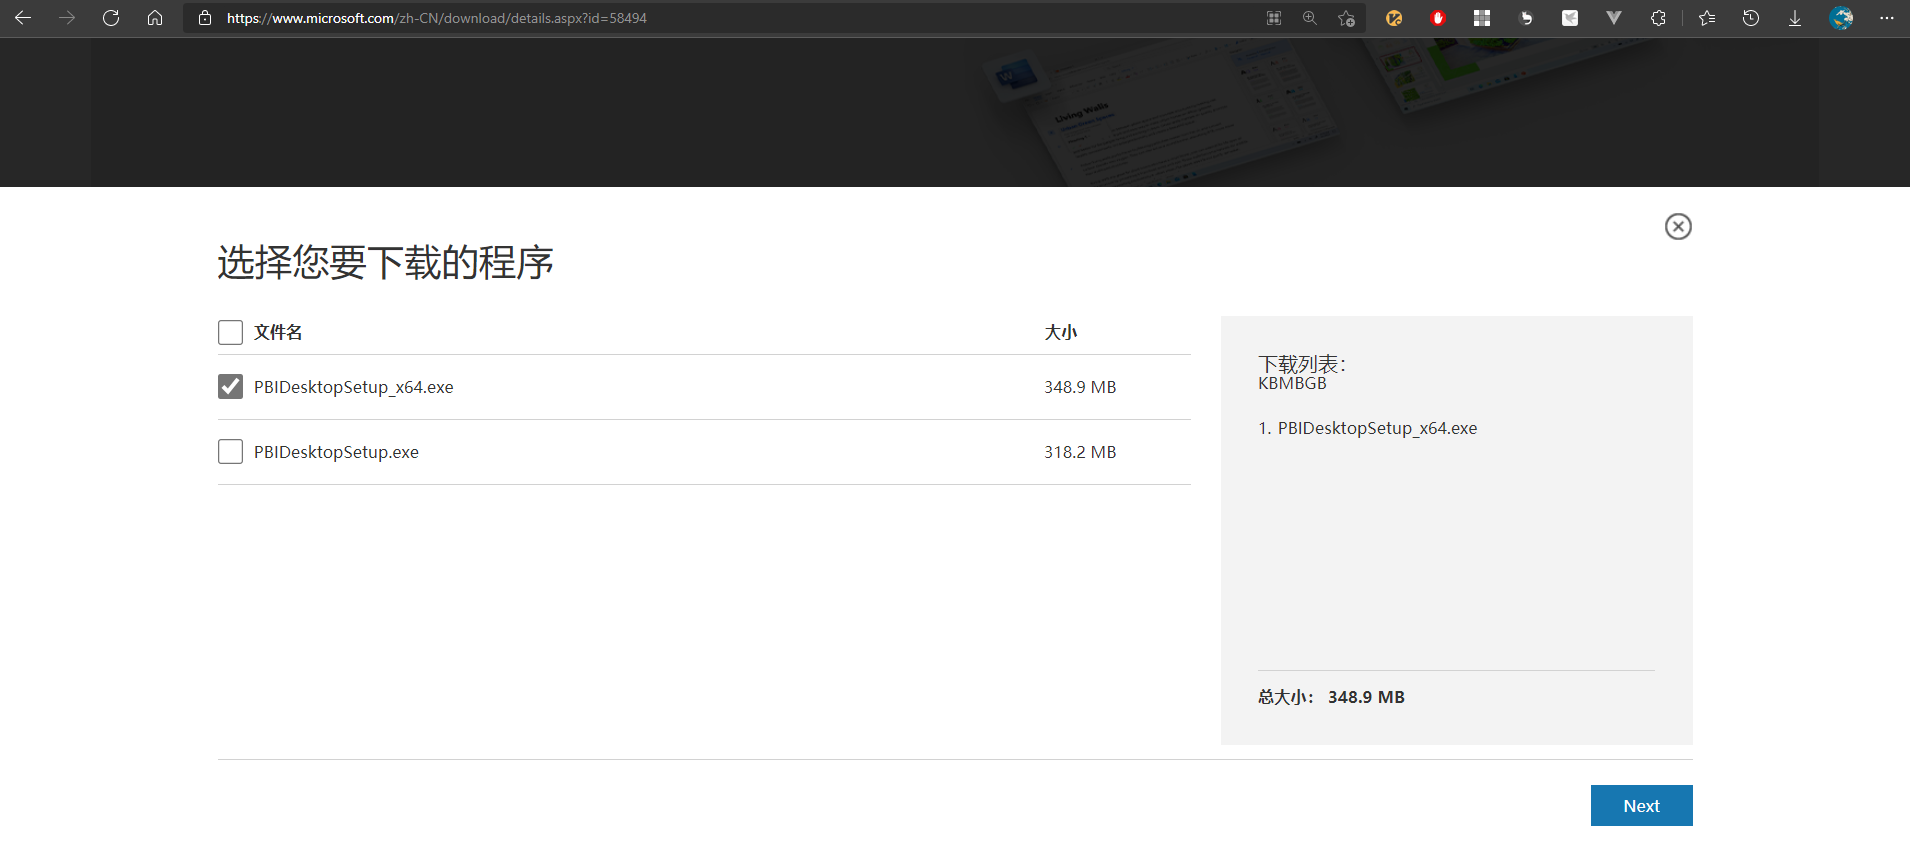
\includegraphics[width=0.9\textwidth]{figure/PowerBI/download_powerbi_web.png}
    \caption{\textbf{从官网下载Power BI Desktop相应版本的安装包}}
    \label{fig:download_powerbi_web}
\end{figure}

注:由于Microsoft Store的网络连接不稳定,更推荐使用方式二,本文中所使用的版本为64位中文版。

安装完成后,启动Power BI Desktop,过程中或会提示登录注册,可使用企业邮箱或学校邮箱进行注册后登录打开Power BI Desktop。也可跳过不注册,但少部分功能会受到影响。

\subsection{认识界面}

如\figref{fig:powerbi_welcome_page}所示,初次启动Power BI Desktop时,会显示欢迎页。从中可以选择获取数据、查看最近使用的源、打开最近的报告以及打开其他报表等。点击右上角的X可关闭欢迎页。

\begin{figure}[htbp]
    \centering
    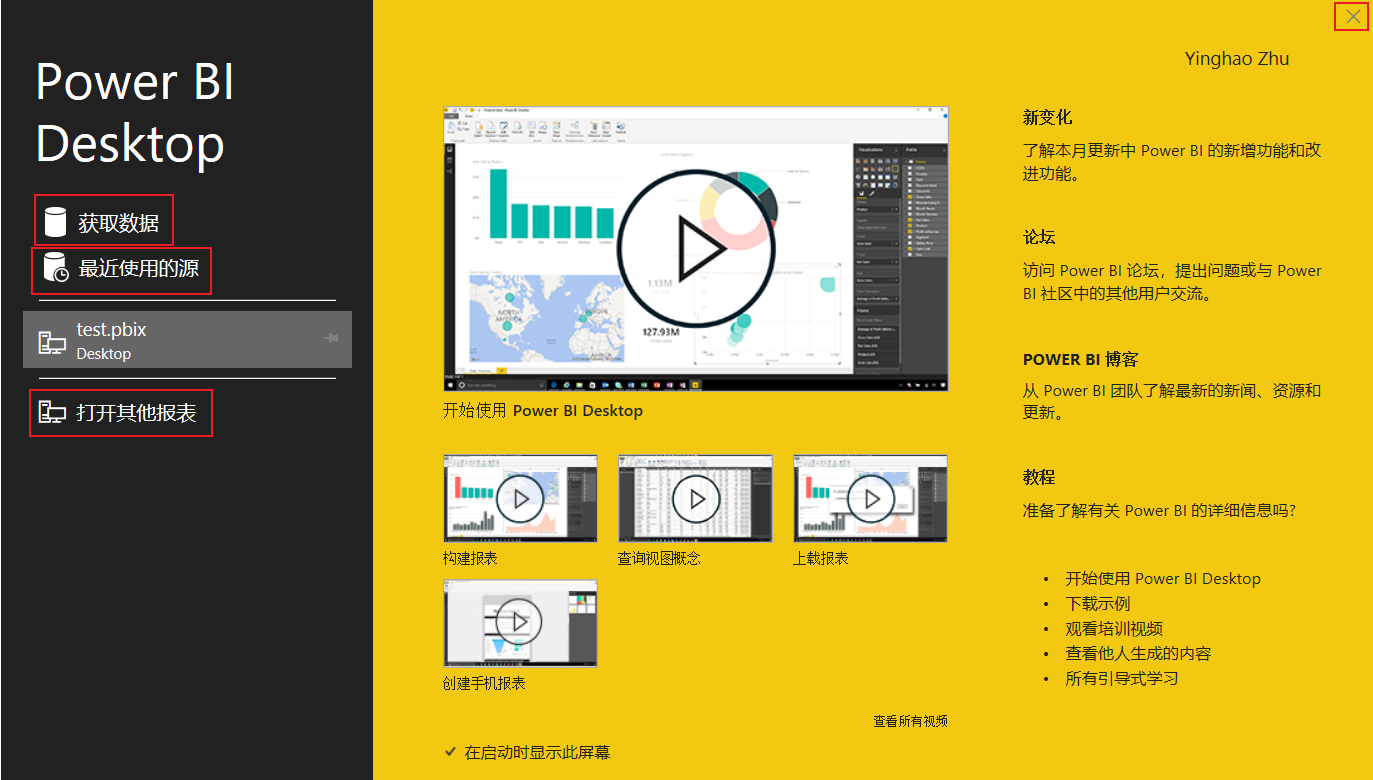
\includegraphics[width=0.7\textwidth]{figure/PowerBI/powerbi_welcome_page.png}
    \caption{\textbf{Power BI Desktop启动时的欢迎页}}
    \label{fig:powerbi_welcome_page}
\end{figure}

Power BI Desktop的界面如\figref{fig:powerbi_ui}中所示,分为了报表视图、数据视图、模型视图、功能区、画布、筛选器、可视化区域、数据字段区域等。

\begin{figure}[htbp]
    \centering
    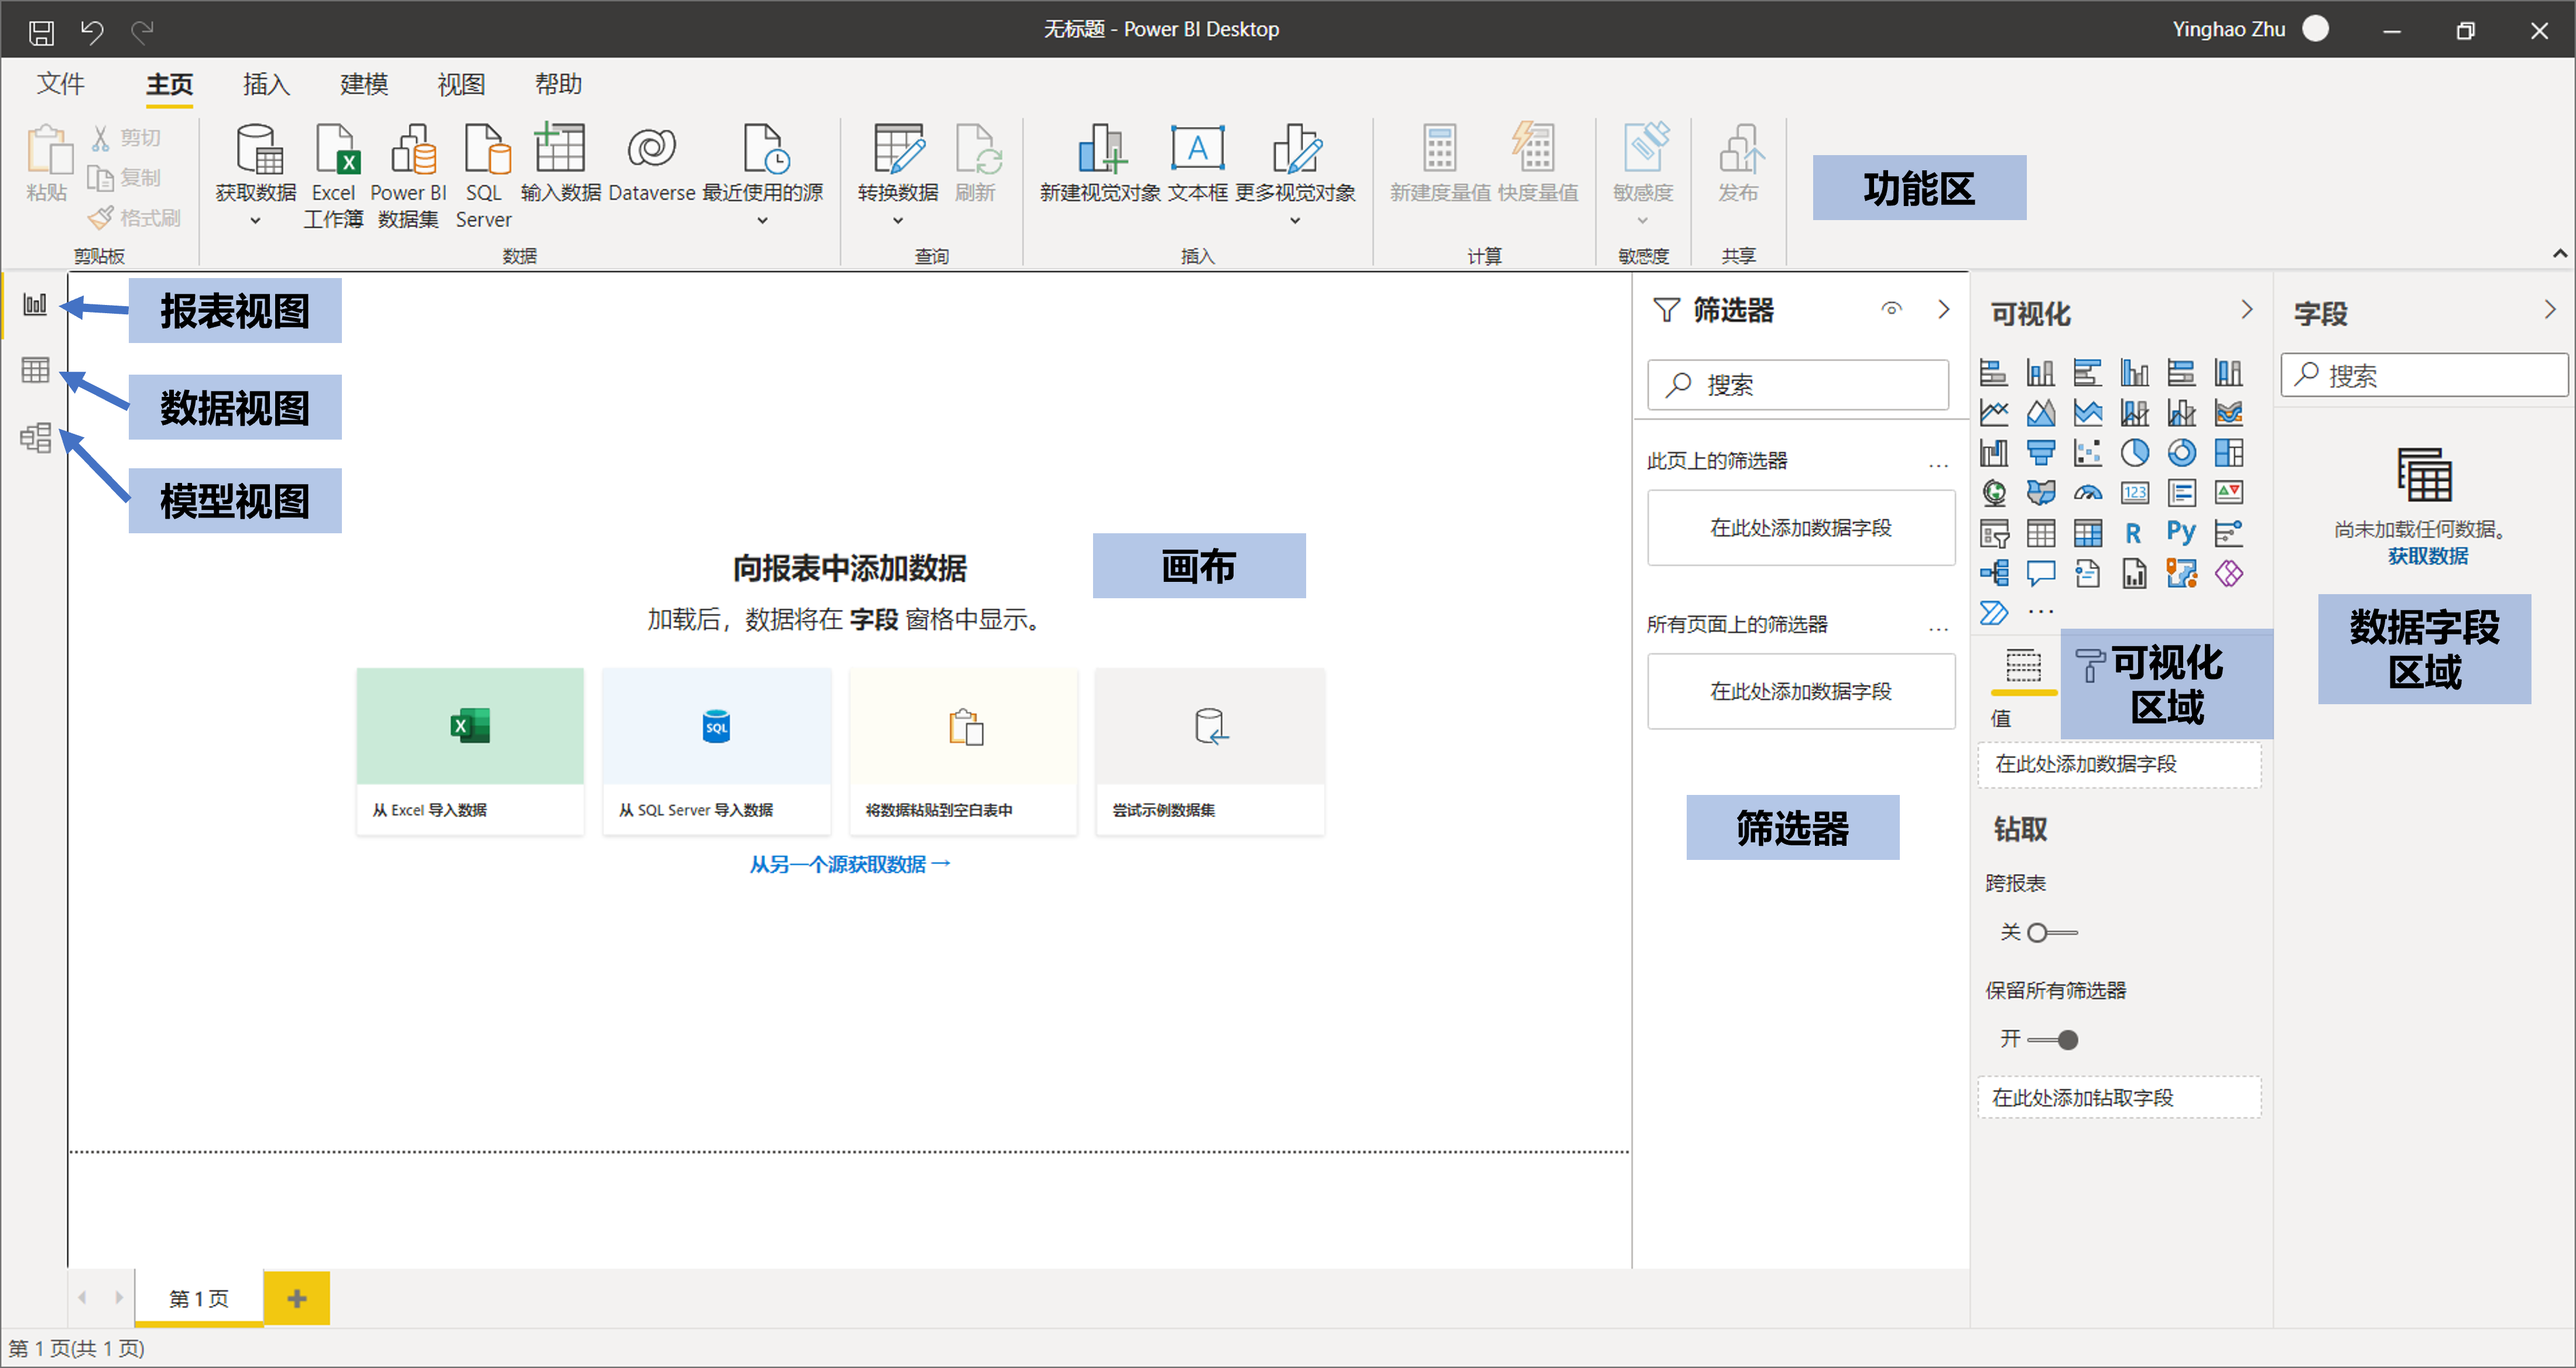
\includegraphics[width=0.9\textwidth]{figure/PowerBI/powerbi_ui.png}
    \caption{\textbf{Power BI Desktop界面}}
    \label{fig:powerbi_ui}
\end{figure}

数据处理的第一步通常为获取外部数据。如\figref{fig:powerbi_load_data}中所示,在工具栏中选择``获取数据'',选择所需的数据来源后即可加载数据。点击``更多'',可选择上百种的数据格式和来源,如Excel、CSV、JSON、SQL Server、MySQL、Spark等,满足主流用户所需。

\begin{figure}[htbp]
    \centering
    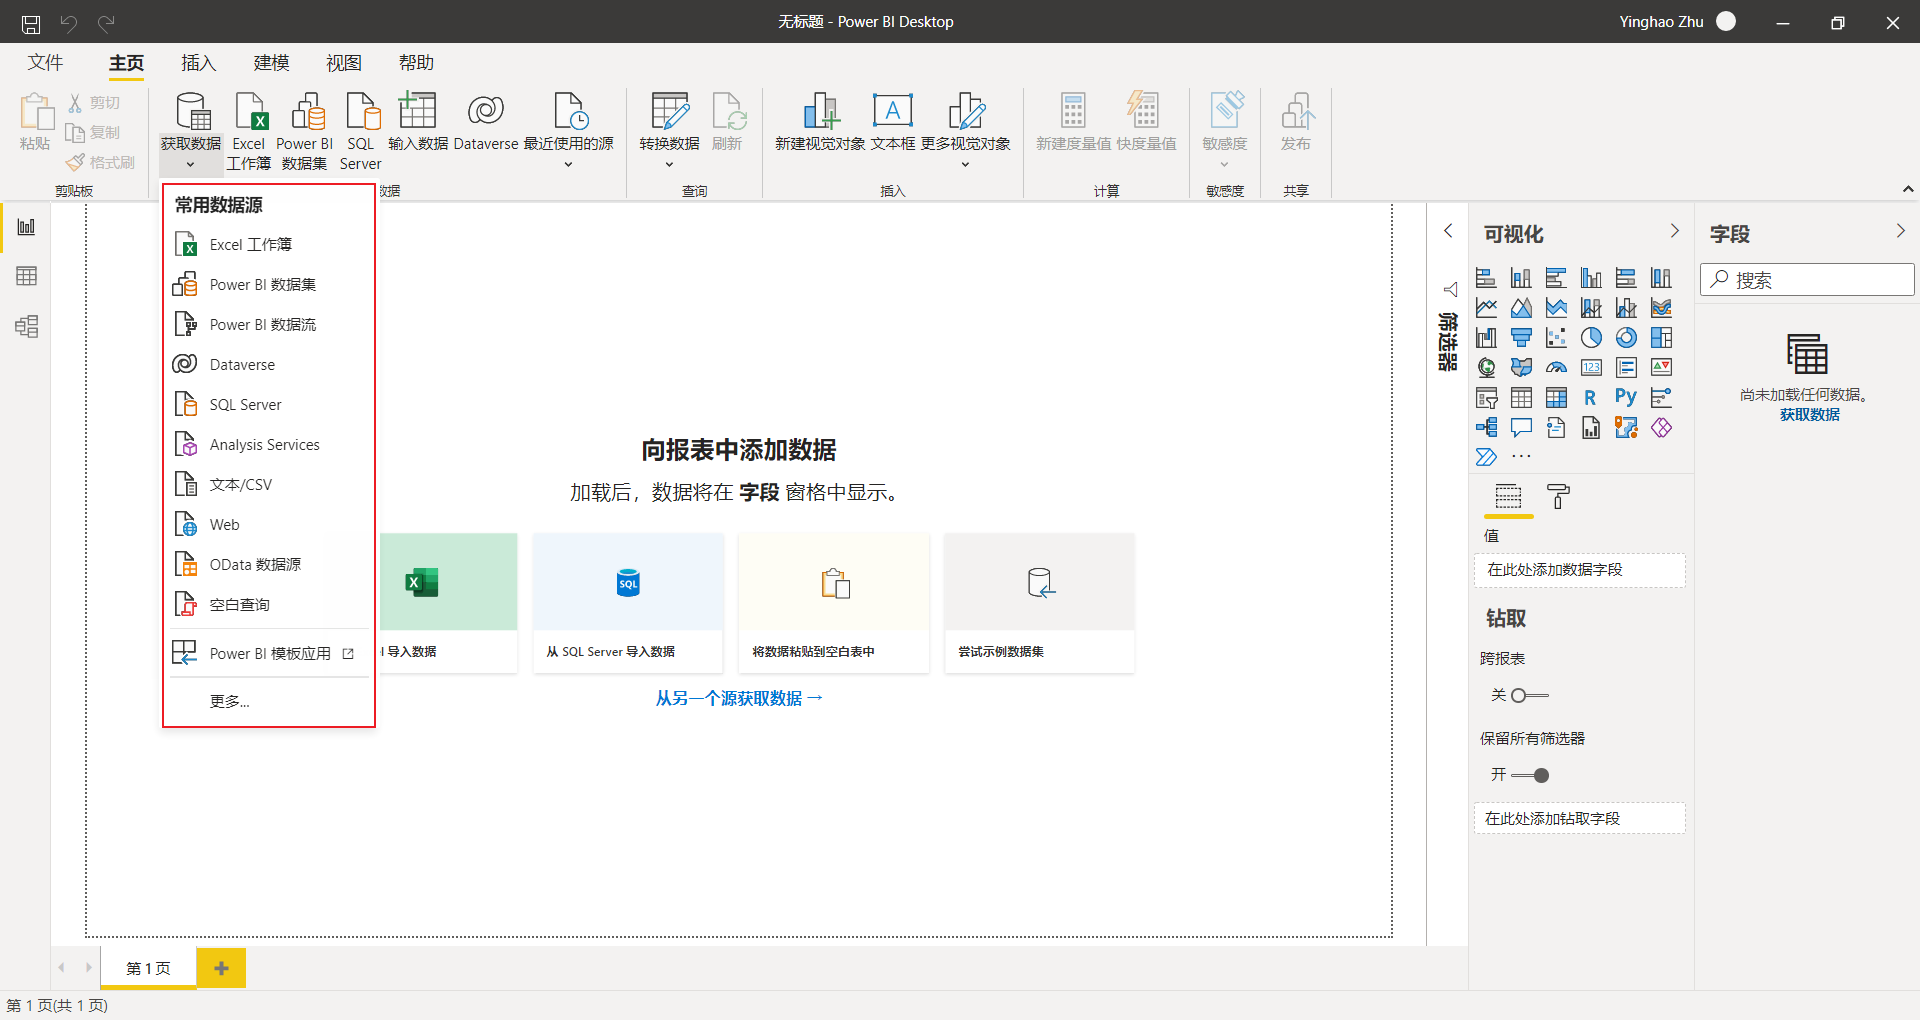
\includegraphics[width=0.9\textwidth]{figure/PowerBI/powerbi_load_data.png}
    \caption{\textbf{选择数据来源,获取数据}}
    \label{fig:powerbi_load_data}
\end{figure}

如\figref{fig:powerbi_sale_profit_graph}所示,以示例数据集Financial Sample.xlsx为例,加载导入数据后,可在字段区域选择希望对比分析的数据字段,此后可视化图表便会在画布中展示出来。此处,我选择了Sales、Date、Profit字段,其默认以柱状图的方式呈现出数据对比图。我们也可以根据数据的特点,在可视化区域内选择其他各种可视化数据方式,如饼图、条形图、环形图等。

\begin{figure}[htbp]
    \centering
    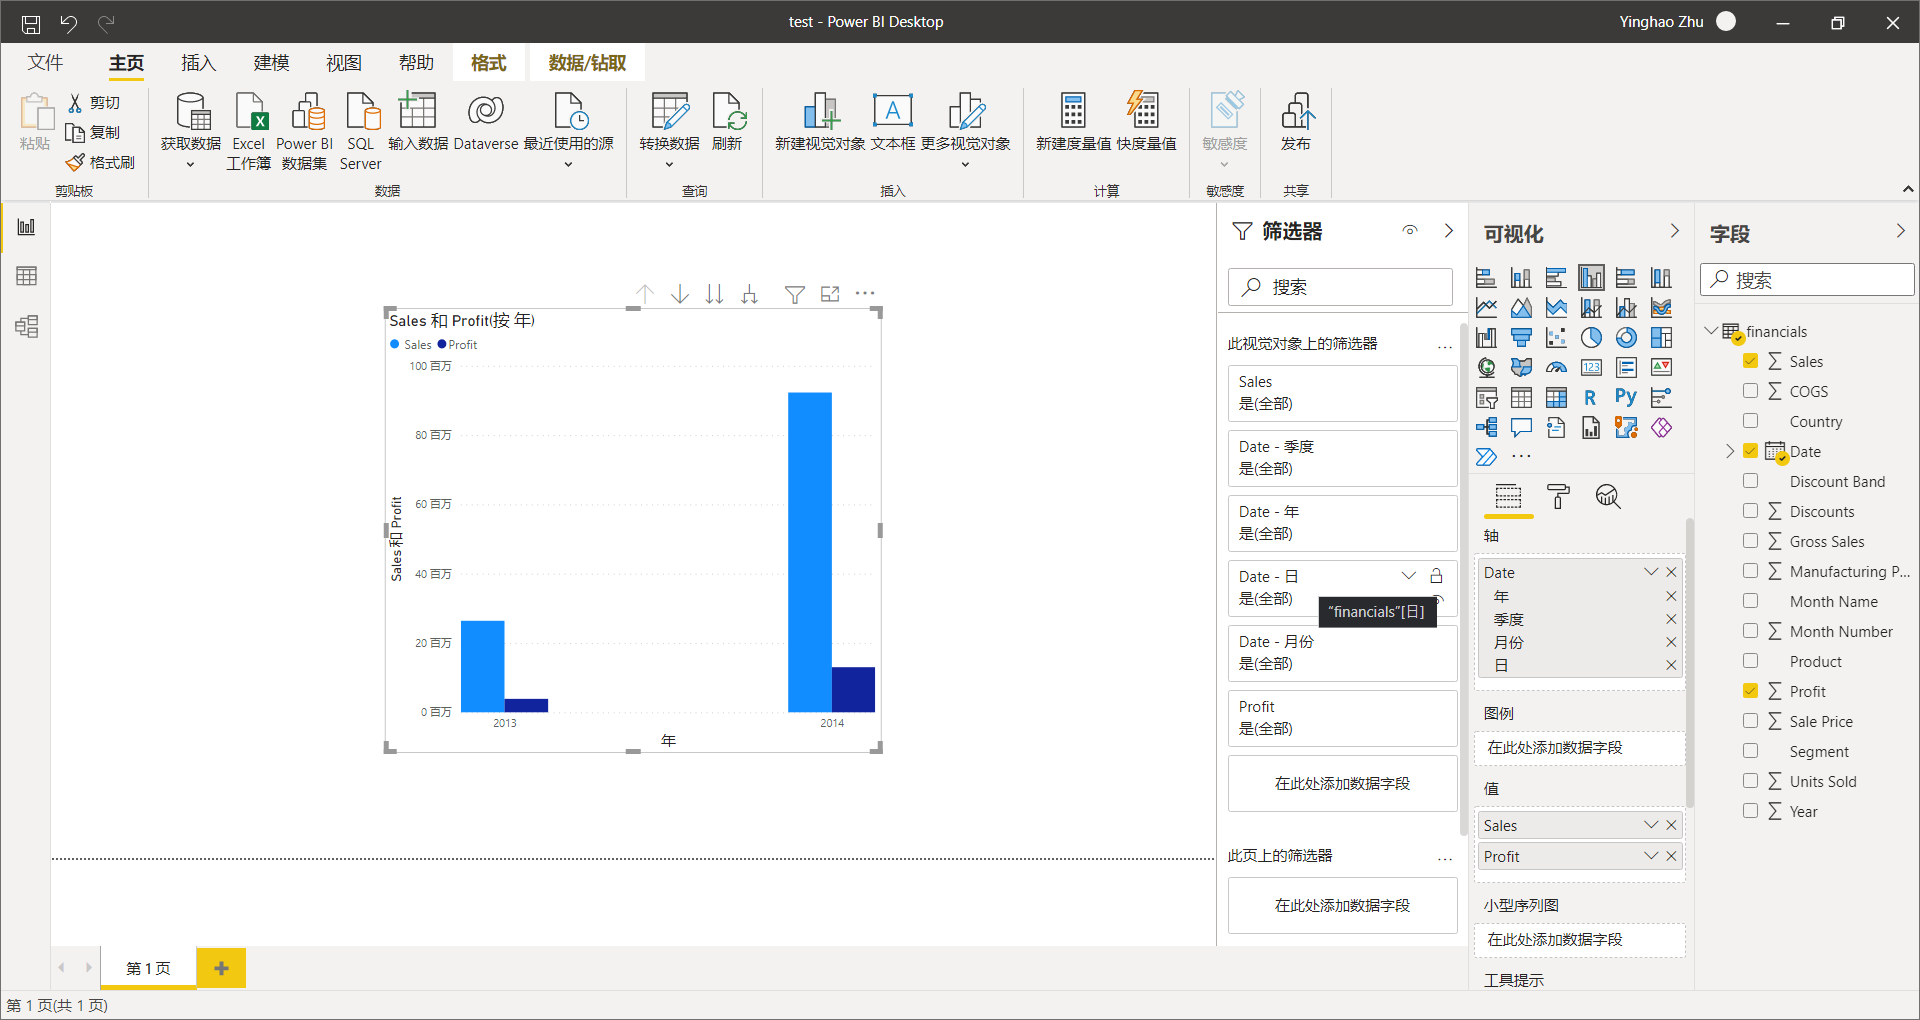
\includegraphics[width=0.9\textwidth]{figure/PowerBI/powerbi_sale_profit_graph.png}
    \caption{\textbf{Financial Sample示例数据集案例}}
    \label{fig:powerbi_sale_profit_graph}
\end{figure}

对于Excel文件等,Power BI提供了内置的Power Query 编辑器。如\figref{fig:powerbi_select_query_editor}所示,鼠标右键字段区域的数据表,选择``编辑查询'',进入到如\figref{fig:powerbi_query_editor_detail}所示中的Power Query编辑器。

\begin{figure}[htbp]
    \centering
    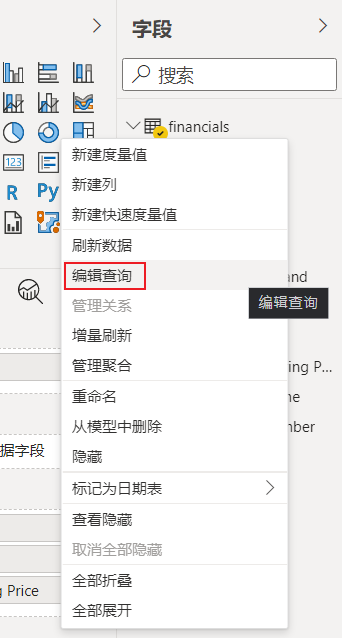
\includegraphics[width=0.4\textwidth]{figure/PowerBI/powerbi_select_query_editor.png}
    \caption{\textbf{右键选择``编辑查询'',进入Power Query 编辑器}}
    \label{fig:powerbi_select_query_editor}
\end{figure}

\begin{figure}[htbp]
    \centering
    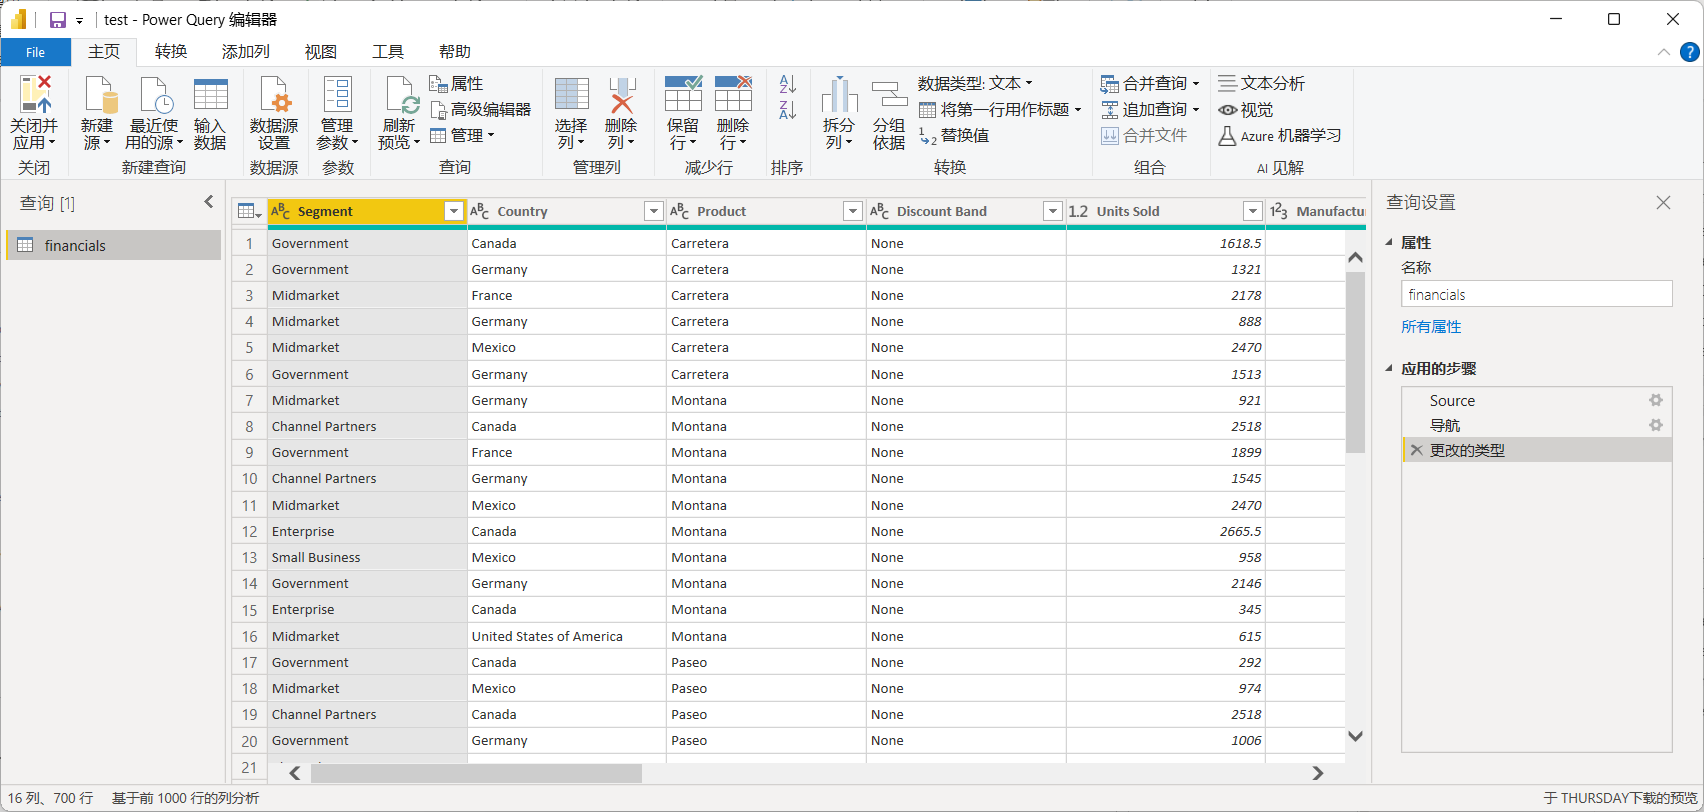
\includegraphics[width=0.9\textwidth]{figure/PowerBI/powerbi_query_editor_detail.png}
    \caption{\textbf{Power Query 编辑器页面}}
    \label{fig:powerbi_query_editor_detail}
\end{figure}

Power Query编辑器是Power BI中的一个非常重要的模块。在Power Query编辑器中,我们可以建立查询和进行数据处理,并将经整理和处理后的数据模型加载至Power BI Desktop中,便于分析和创建报表。

我们点击Power BI Desktop左侧的侧边栏,切换不同的视图。默认为如\figref{fig:powerbi_sale_profit_graph}所示中的报表视图,我们可以切换至如\figref{fig:powebi_data_view}所示中的数据视图,查看经过Power Query编辑器中整理得到的数据。此外,还可以切换至模型视图。

\begin{figure}[htbp]
    \centering
    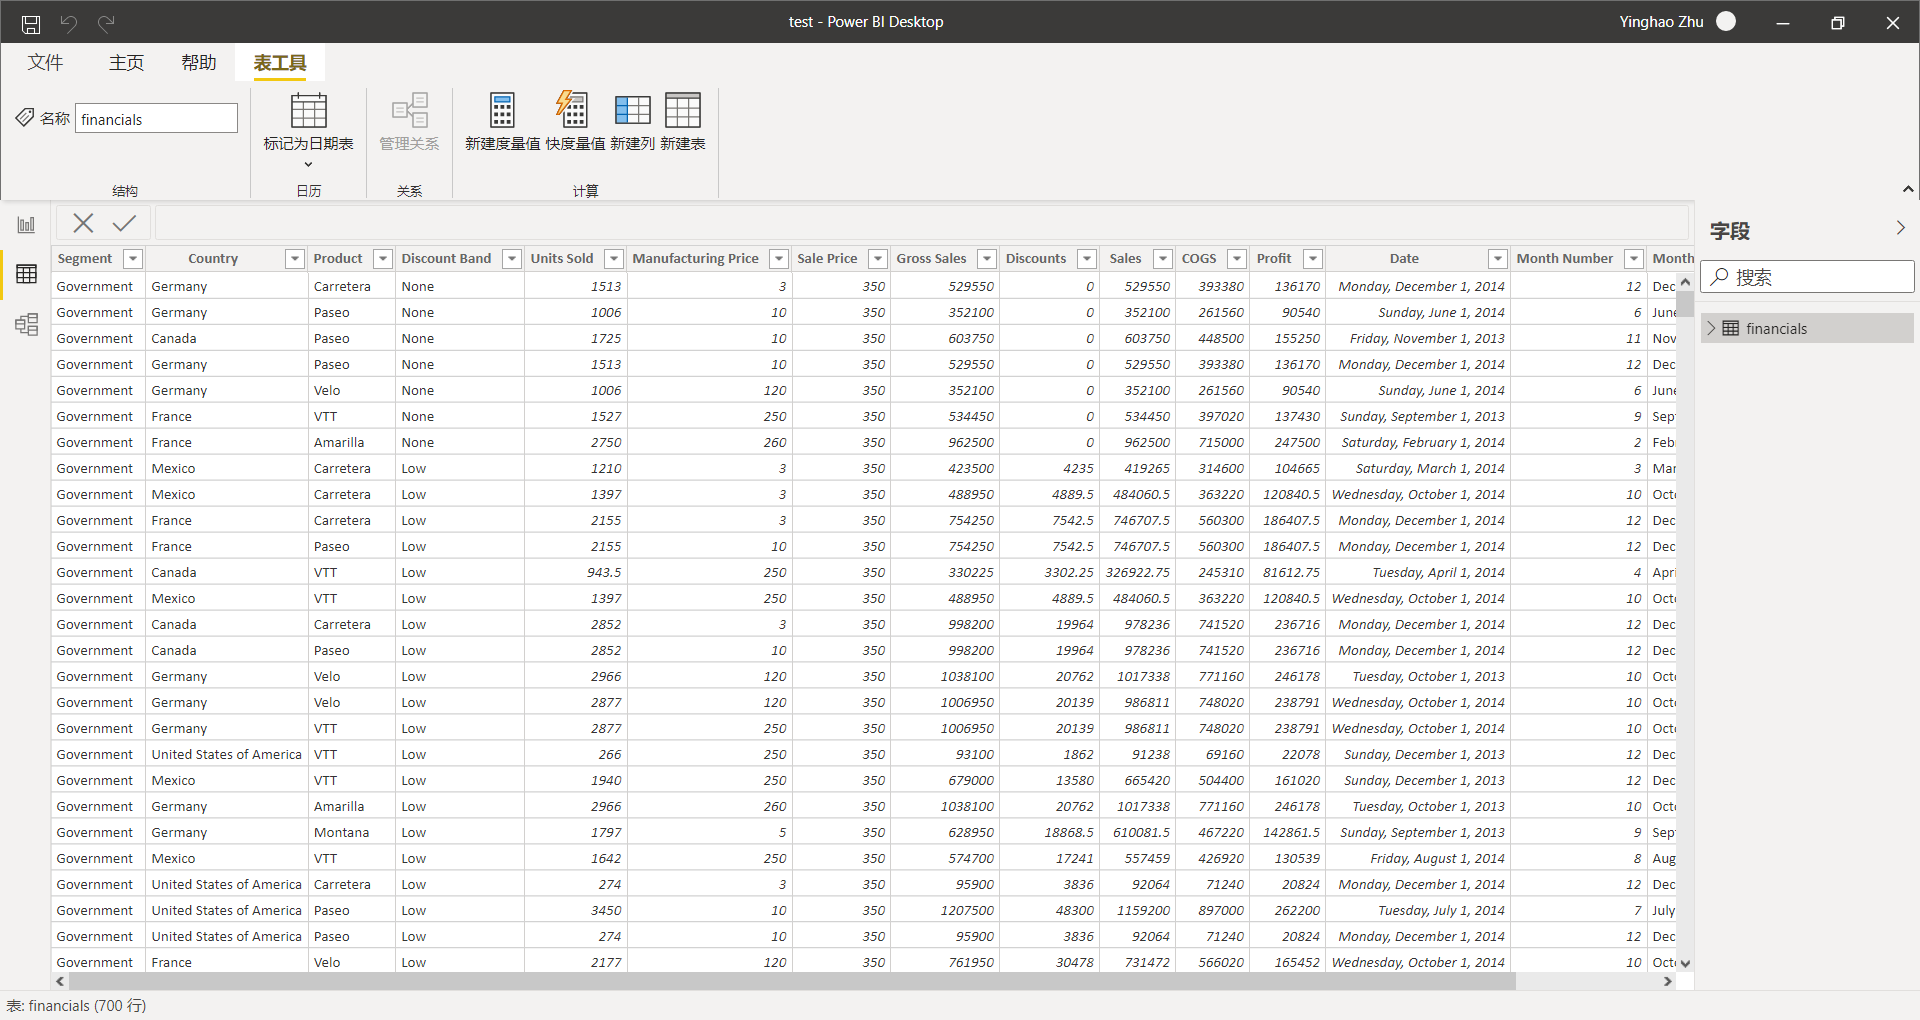
\includegraphics[width=0.9\textwidth]{figure/PowerBI/powerbi_data_view.png}
    \caption{\textbf{数据视图页面}}
    \label{fig:powebi_data_view}
\end{figure}